\documentclass[aspectratio=169]{beamer}

\usetheme{Warsaw}
\usecolortheme{default}

\usepackage[T1]{fontenc}
\usepackage{lmodern}
\usepackage{graphicx}
\usepackage{booktabs}
\usepackage{xcolor}

\definecolor{PUT-blue}{RGB}{0,84,147}
\definecolor{PUT-dark}{RGB}{0,45,85}
\definecolor{highlight}{RGB}{230,126,34}
\definecolor{commentbg}{RGB}{245,248,252}

\setbeamercolor{palette primary}{bg=PUT-blue,fg=white}
\setbeamercolor{palette secondary}{bg=PUT-dark,fg=white}
\setbeamercolor{palette tertiary}{bg=PUT-blue,fg=white}
\setbeamercolor{structure}{fg=PUT-blue}
\setbeamertemplate{headline}{}
\setbeamertemplate{footline}{%
  \leavevmode%
  \hbox{%
    \begin{beamercolorbox}[
      wd=.40\paperwidth,
      ht=2.75ex,
      dp=1.125ex,
      left,
      leftskip=.4cm,
      rightskip=.3cm
    ]{author in head/foot}%
      \usebeamerfont{author in head/foot}\insertshortauthor%
    \end{beamercolorbox}%
    \begin{beamercolorbox}[
      wd=.48\paperwidth,
      ht=2.75ex,
      dp=1.125ex,
      left,
      leftskip=.3cm,
      rightskip=.15cm
    ]{title in head/foot}%
      \usebeamerfont{title in head/foot}\insertshorttitle%
    \end{beamercolorbox}%
    \begin{beamercolorbox}[
      wd=.12\paperwidth,
      ht=2.75ex,
      dp=1.125ex,
      right,
      leftskip=.15cm,
      rightskip=.4cm
    ]{title in head/foot}%
      \usebeamerfont{title in head/foot}\insertframenumber/\inserttotalframenumber%
    \end{beamercolorbox}%
  }%
}

\graphicspath{{../notebooks/plots/}}

\newcommand{\slidecomment}[1]{
    \vspace{0.3em}
    \begin{beamercolorbox}[wd=\linewidth,rounded=true,sep=0.7ex]{block body}
        \small #1
    \end{beamercolorbox}
}

\title{Kaggle TensorFlow Speech Recognition Challenge}
\author{Paweł Pozorski \and Paweł Florek}
\institute{Warsaw University of Technology}
\date{\today}

\begin{document}

\begin{frame}[plain]
    \titlepage
\end{frame}

\begin{frame}{Agenda}
    \tableofcontents
\end{frame}

\section{Problem and Setup}

\begin{frame}{Task Formulation}
    \begin{itemize}
        \item Dataset: Kaggle TensorFlow Speech Recognition (Google Speech Commands v1 derivative).
        \item Fixed 12-class setup: 10 commands + \texttt{\_\_unknown\_\_} + \texttt{\_\_silence\_\_}.
        \item Strict 4-phase funnel: feature selection, optimization tuning, architecture comparison, open-set strategy comparison.
        \item Three fixed seeds for every configuration for stability estimates.
    \end{itemize}
\end{frame}

\begin{frame}{Dataset Splits and Evaluation Protocol}
    \begin{itemize}
        \item \textbf{Phases 1--3:} command-only small splits (\texttt{train\_small}, \texttt{valid\_small}, \texttt{test\_small}).
        \item \textbf{Phase 4:} extended 12-class splits with explicit unknown/silence handling.
        \item \textbf{Seeds:} 3 fixed seeds (\(0,42,2003\)) for each configuration.
        \item \textbf{Selection rule:} preserve command quality first, then optimize non-command robustness.
    \end{itemize}
\end{frame}

\begin{frame}{Stage-Wise Architectures and Approaches}
    \small
    \begin{itemize}
        \item \textbf{Stage 1 (Feature selection):} comparison on \textbf{ConvNeXt + xLSTM} across mel/mfcc/pcen/specaugment pipelines.
        \item \textbf{Stage 2 (Global tuning):} same proxy families with \textbf{scheduler + weight decay} sweep (cosine warmup vs reduce-on-plateau).
        \item \textbf{Stage 3 (Architecture comparison):} full comparison of \textbf{ConvNeXt, AST, MLP-Mixer} (SSAMBA/xLSTM kept as planned, not executed).
        \item \textbf{Stage 4 (Open-set handling):} top backbones retrained with \textbf{flat multiclass, sampling control, loss reweighting, two-stage}.
    \end{itemize}
\end{frame}

\begin{frame}{Models and Methods}
    \small
    \textbf{Feature strategies (Stage 1)}
    \begin{itemize}
        \item \textbf{Mel-spectrogram:} log-mel time-frequency baseline representation.
        \item \textbf{High-temporal mel:} shorter window/hop for denser time sampling.
        \item \textbf{MFCC:} DCT-compressed mel representation with lower dimensionality.
        \item \textbf{PCEN:} adaptive per-channel normalization emphasizing transients.
        \item \textbf{Mel + SpecAugment:} mel features with time/frequency masking during training.
    \end{itemize}
\end{frame}

\begin{frame}{Models and Methods}
    \small
    \textbf{Model families}
    \begin{itemize}
        \item \textbf{ConvNeXt (CNN):} convolutional hierarchy for local time-frequency pattern extraction, with modern architectural improvements (transformer approach).
        \item \textbf{AST (Transformer):} self-attention over spectrogram patches for global context modeling.
        \item \textbf{MLP-Mixer:} MLP-only token/channel mixing without convolution or attention blocks.
    \end{itemize}
    \vspace{0.2em}
    \textbf{Planned but unused in executed Stage 3}
    \begin{itemize}
        \item \textbf{xLSTM}: recurrent sequence model, used in early stages and kept in repository scope, dropped due to poor performance.
        \item \textbf{SSAMBA/Mamba}: selective state-space sequence model, implemented but not part of executed Stage 3 runs due to computational constraints.
    \end{itemize}
    \vspace{0.2em}
\end{frame}

\begin{frame}{Models and Methods}
    \small
    \textbf{Open-set methods (Phase 4)}
    \begin{itemize}
        \item \textbf{Flat multiclass:} one classifier over 12 labels.
        \item \textbf{Sampling control:} weighted batch sampling with predefined class priors.
        \item \textbf{Loss reweighting:} class-weighted cross-entropy to rebalance training signal.
        \item \textbf{Two-stage detector:} binary command/non-command gate plus specialist branches.
    \end{itemize}
\end{frame}

\section{Results by Phase}

\begin{frame}{Phase 1: Feature Pipeline vs Model Family}
    \centering
    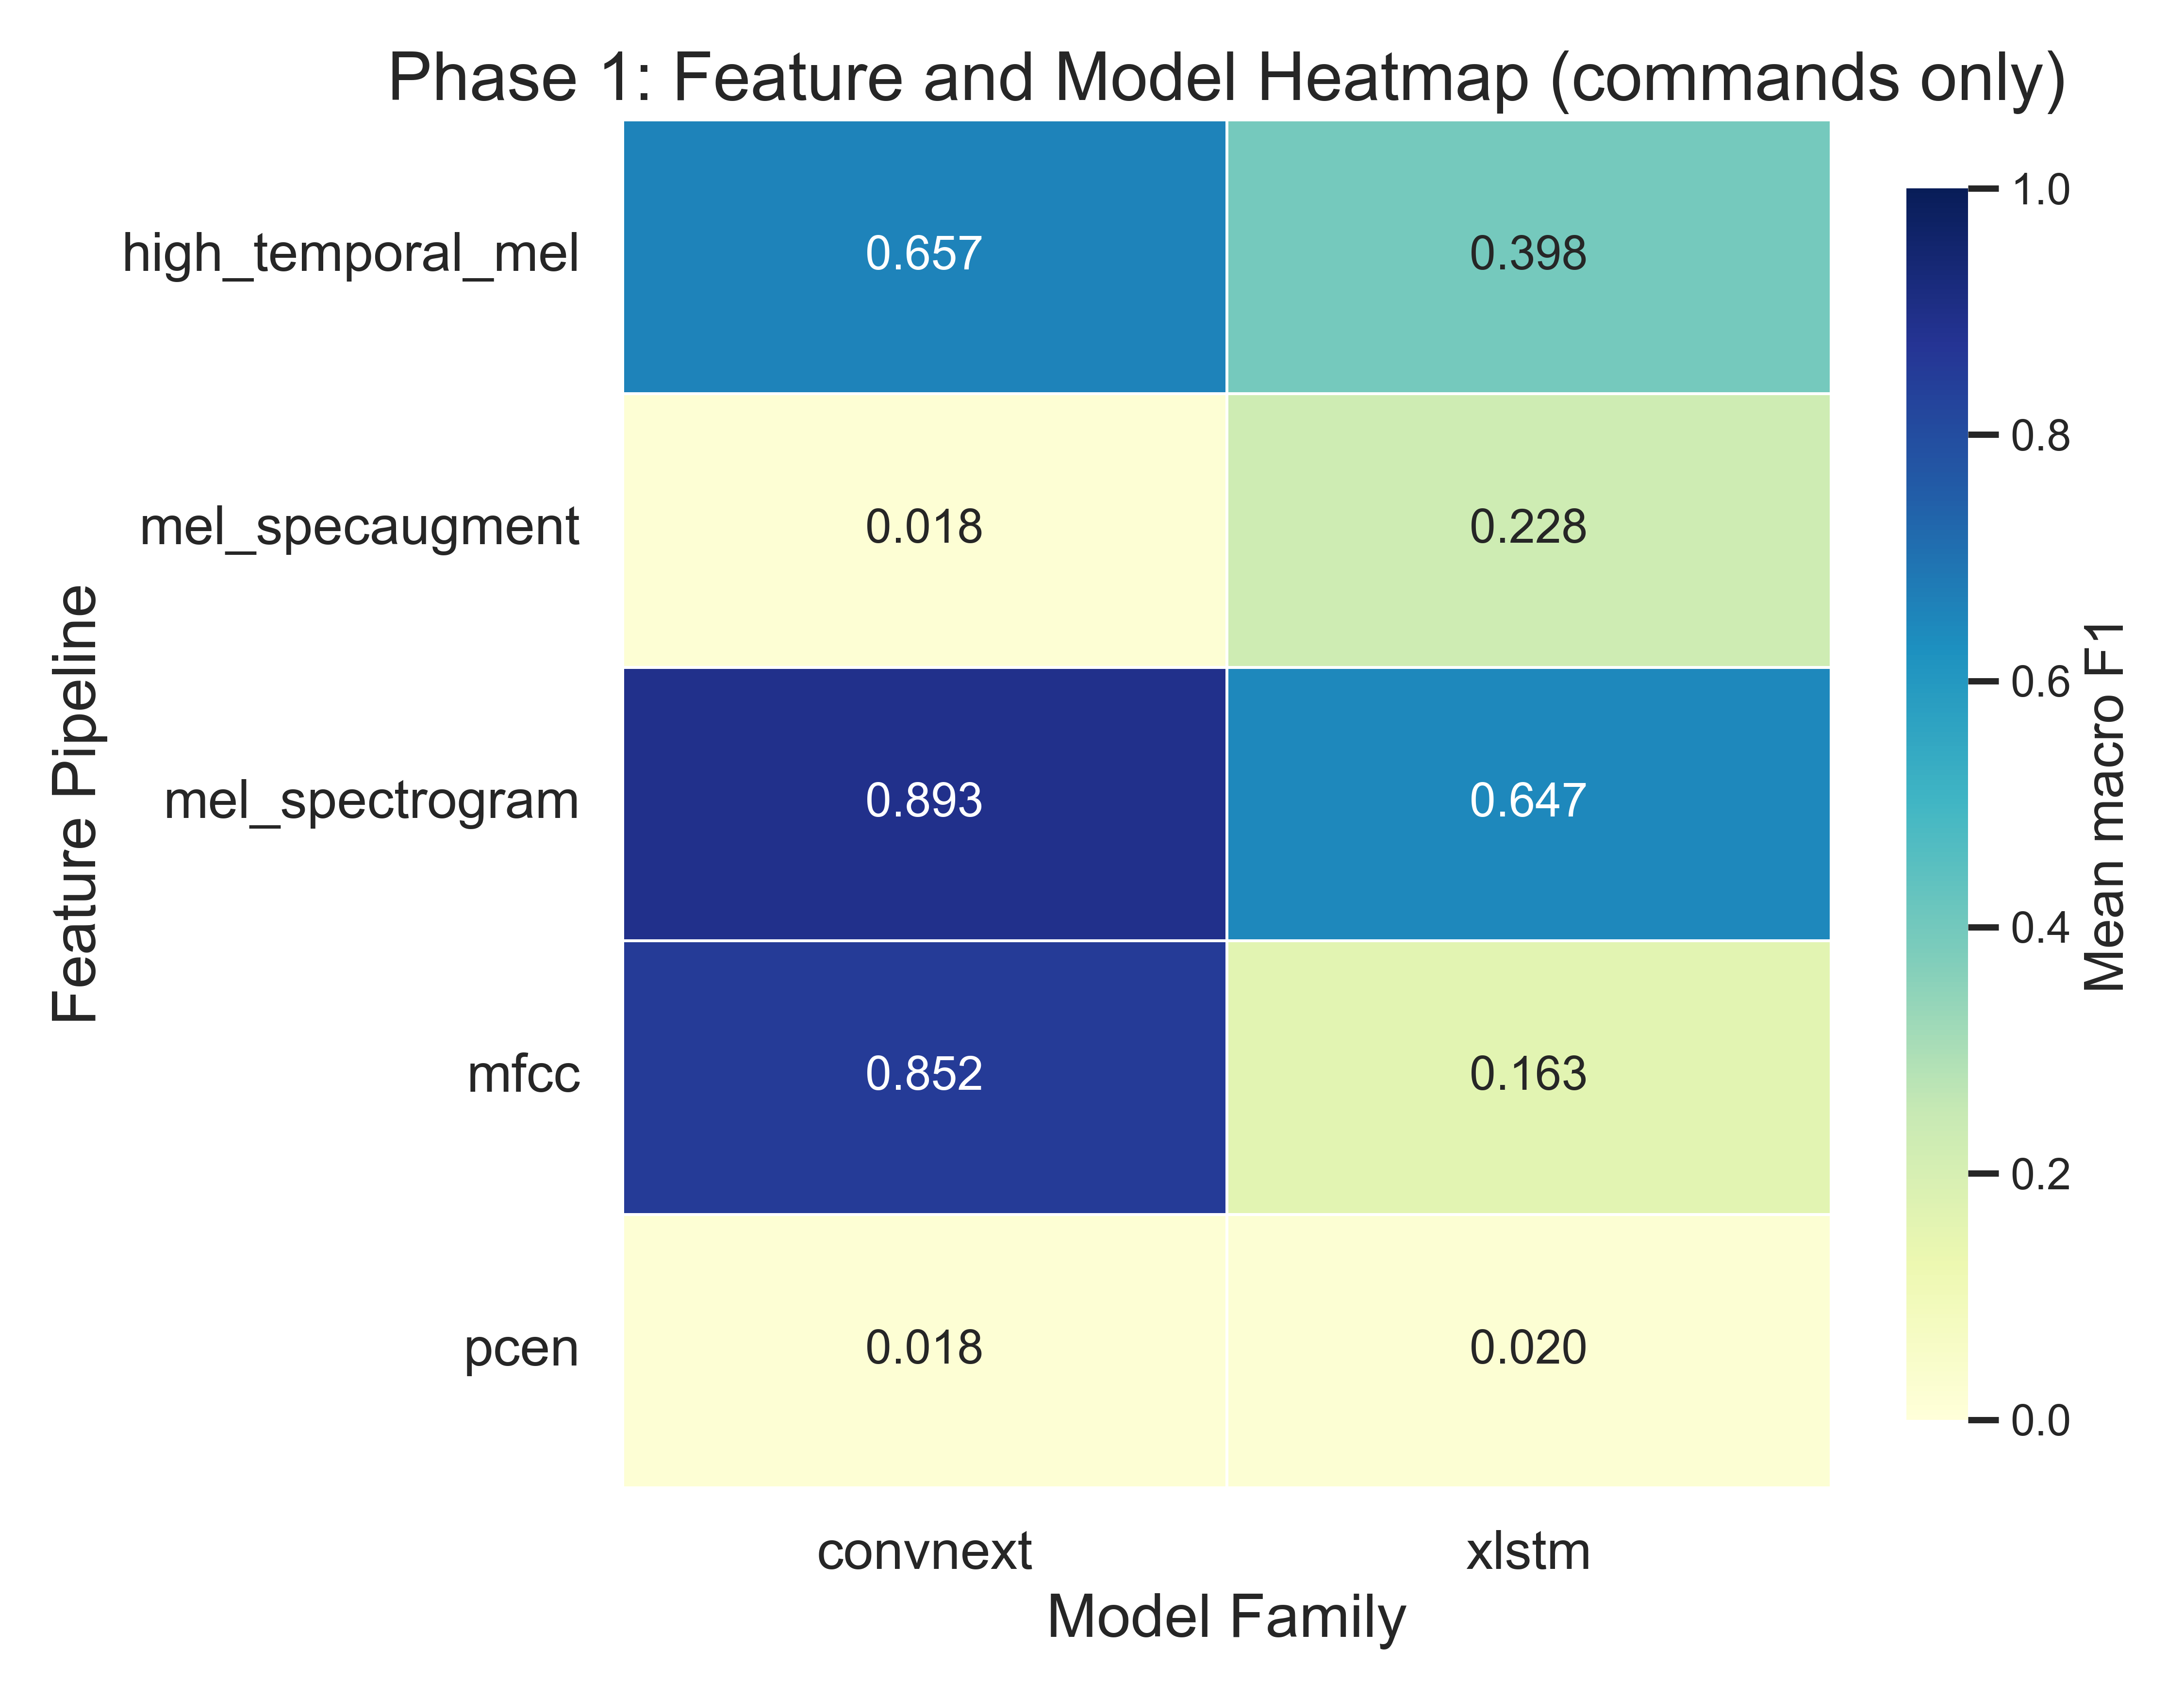
\includegraphics[height=0.70\textheight,keepaspectratio]{phase_1_heatmap.png}
    \slidecomment{Mel-based front ends (including MFCC) are strongest overall; xLSTM underperforms expectations and is dropped later.}
\end{frame}

\begin{frame}{Phase 2: Regularization Sensitivity}
    \centering
    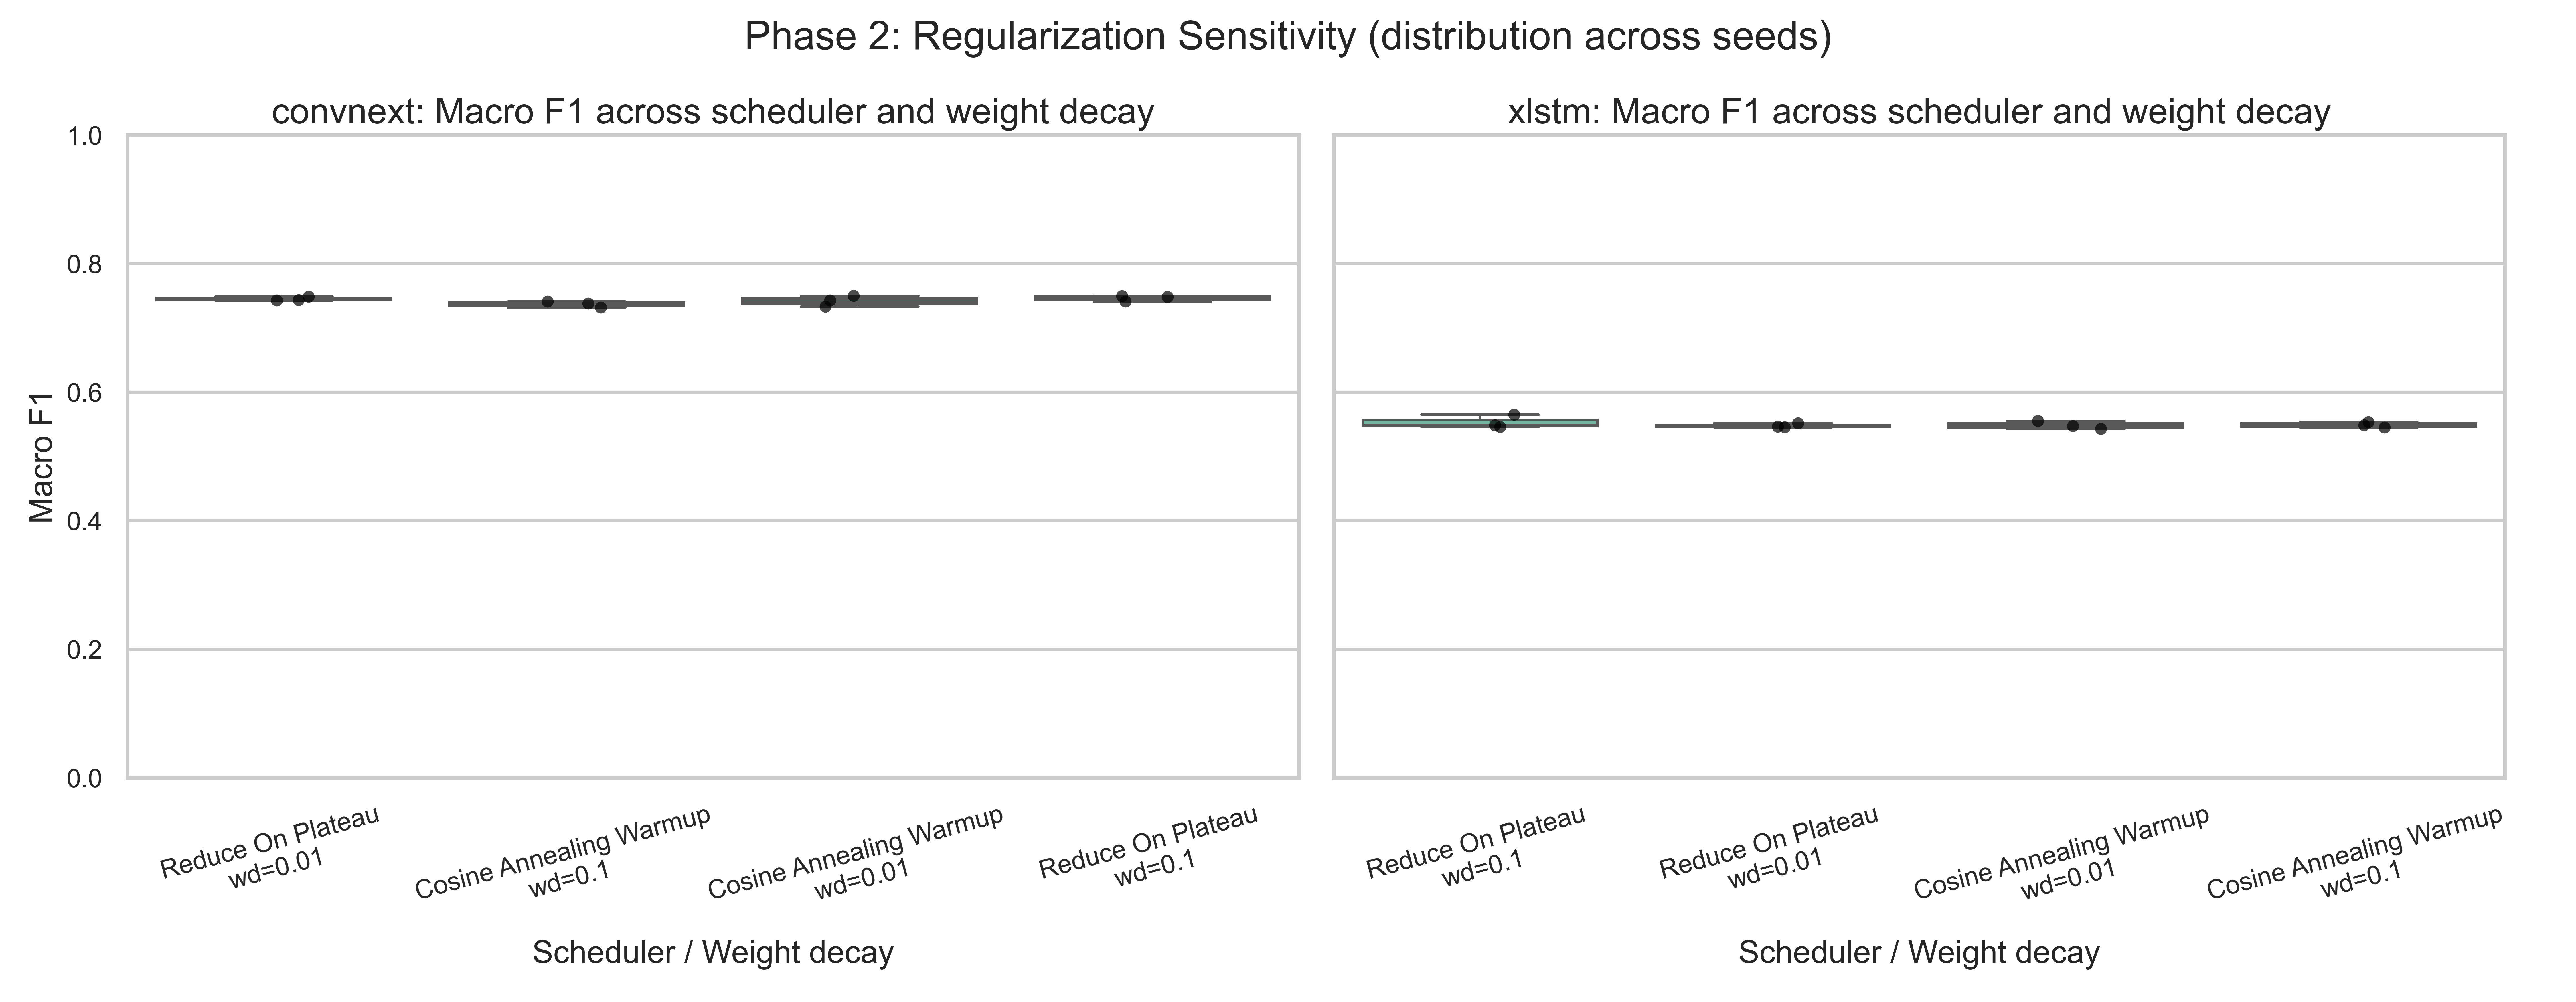
\includegraphics[height=0.68\textheight,keepaspectratio]{phase_2_regularization_sensitivity_2col.png}
    \slidecomment{Most optimizer/scheduler settings are close in F1.}
\end{frame}

\begin{frame}{Phase 2: Convergence Speed}
    \centering
    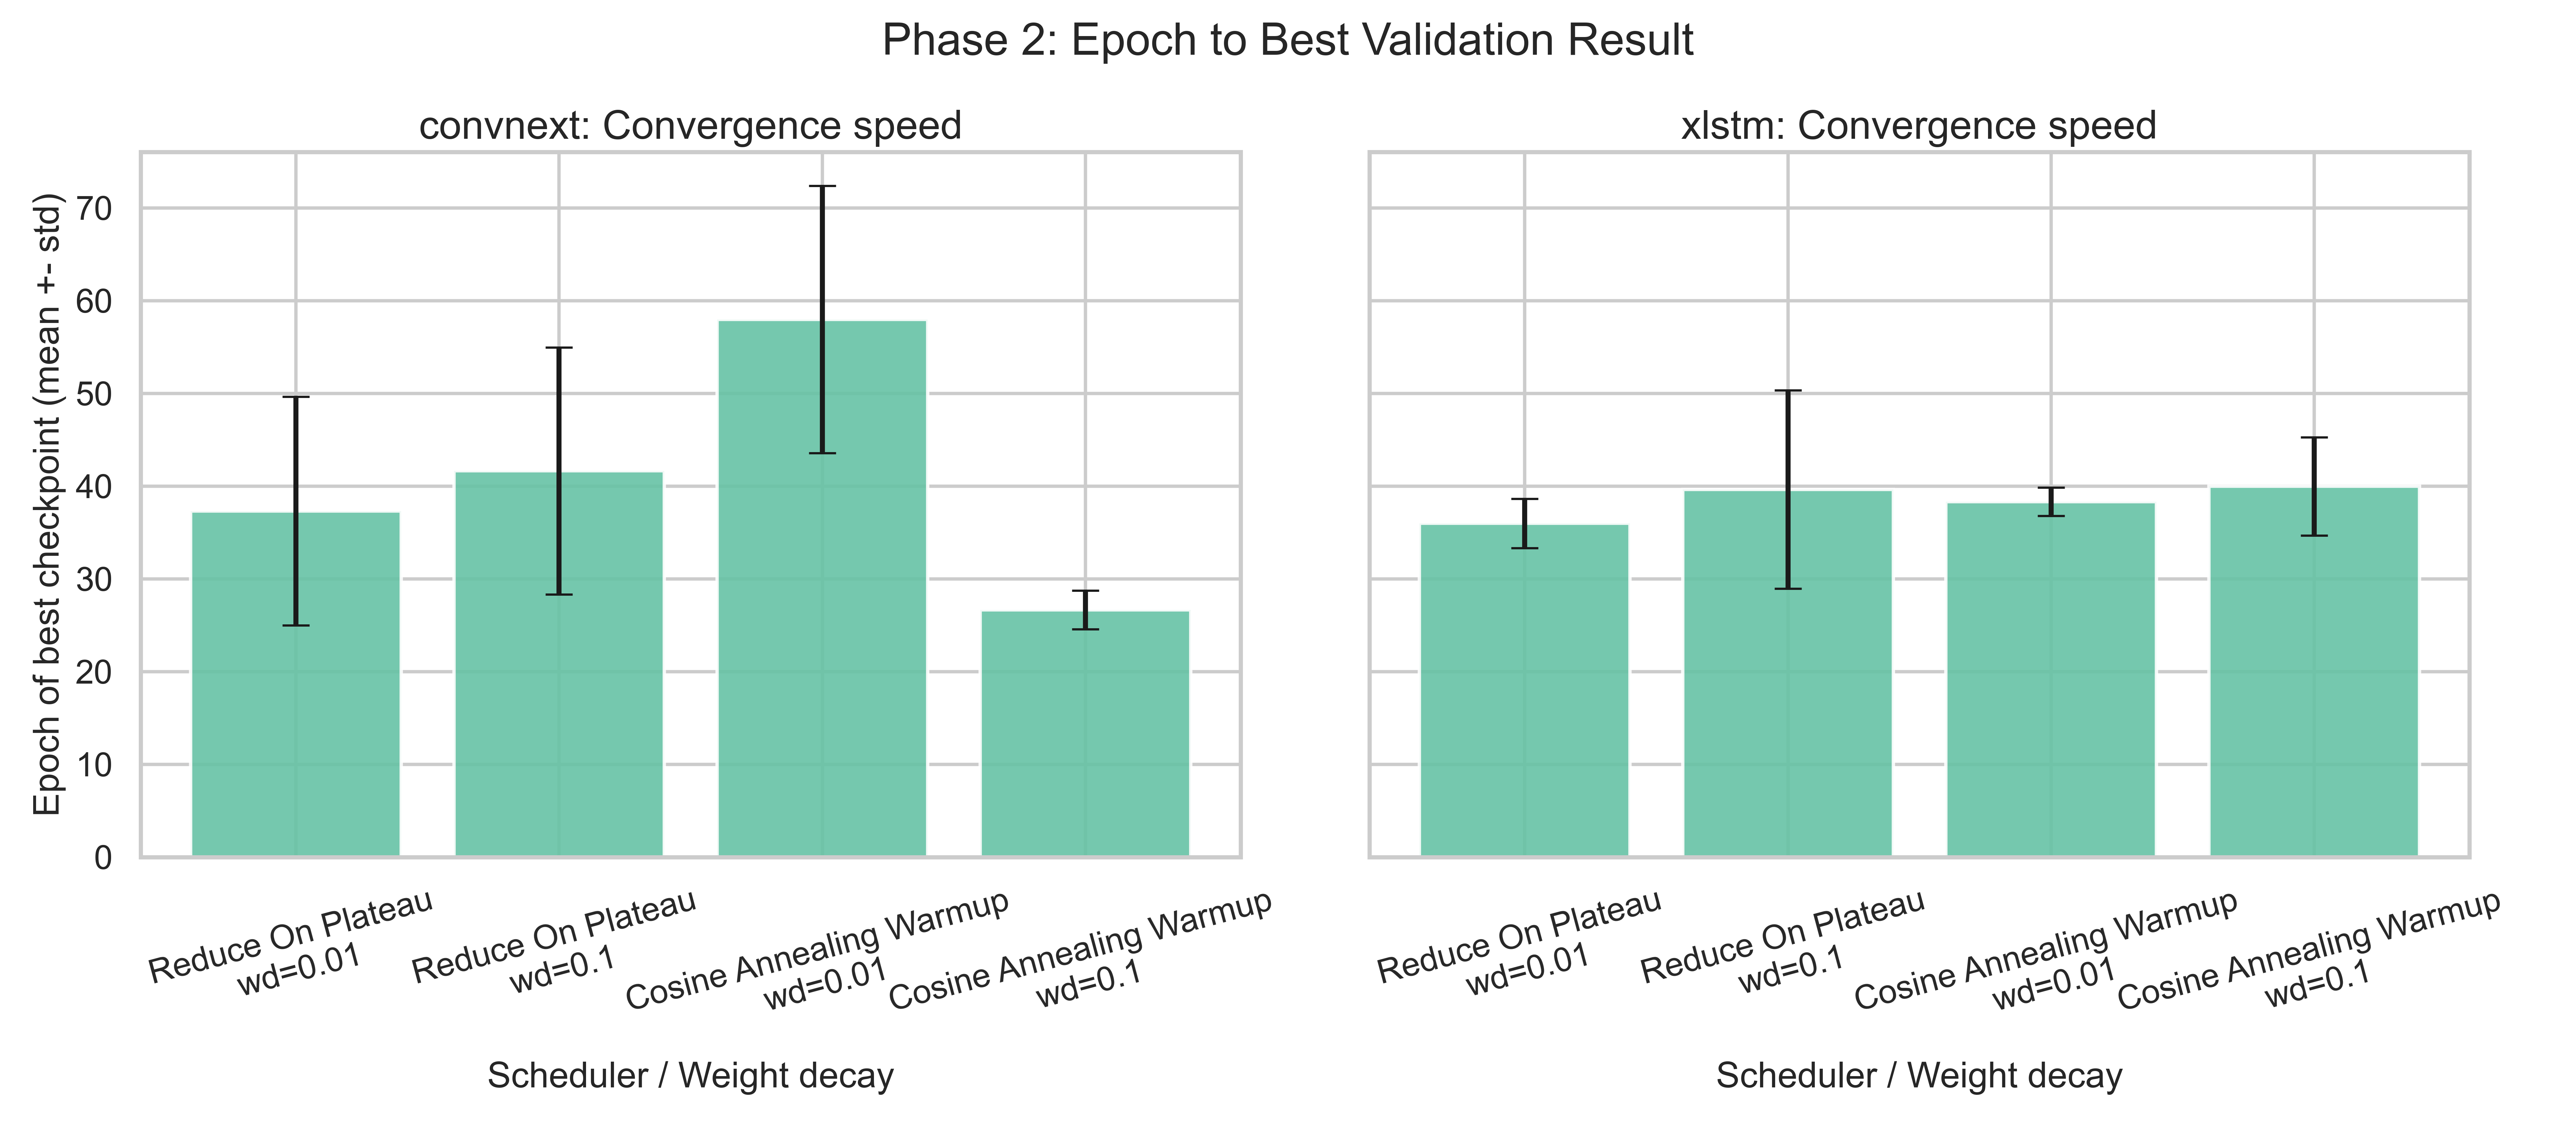
\includegraphics[height=0.68\textheight,keepaspectratio]{phase_2_convergence_speed_2col.png}
    \slidecomment{Cosine annealing with warmup and stronger weight decay gives the best convergence-quality trade-off for the winning branch (on ConvNeXt).}
\end{frame}

\begin{frame}{Phase 3: Architecture Distribution}
    \centering
    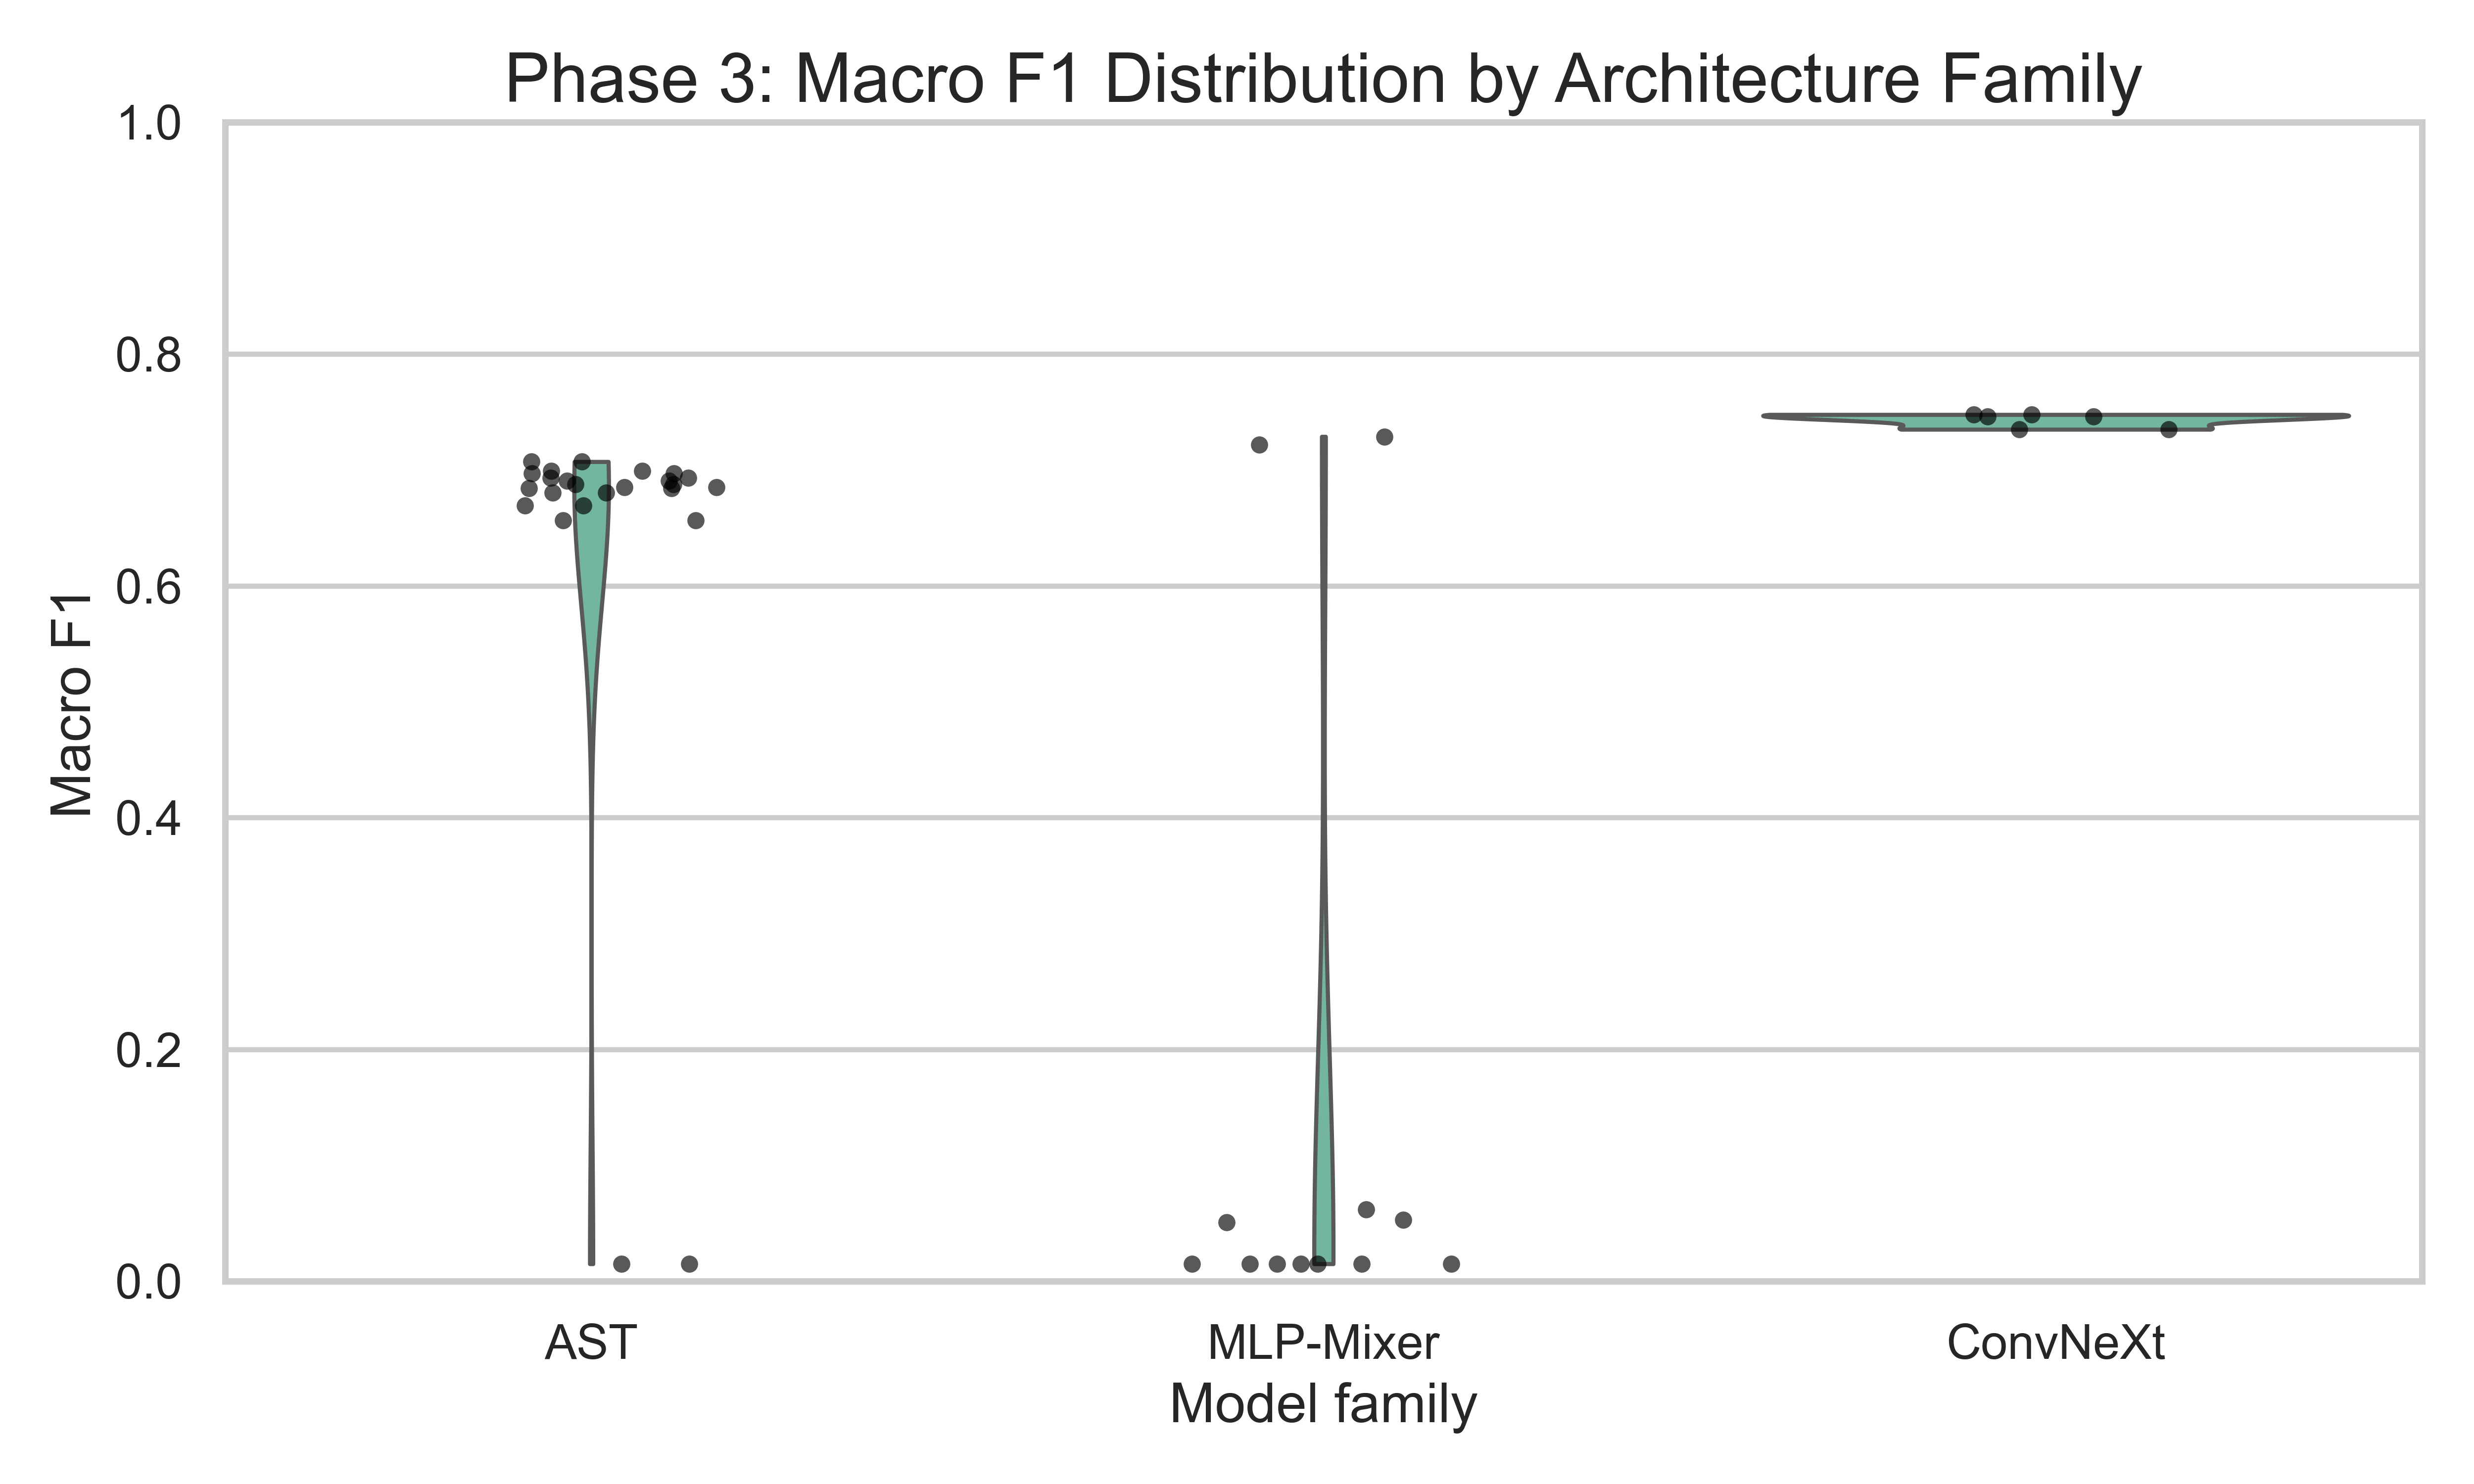
\includegraphics[height=0.68\textheight,keepaspectratio]{phase_3_architecture_distribution.png}
    \slidecomment{ConvNeXt is best and most stable; AST is competitive but less stable; MLP-Mixer is consistently weaker.}
\end{frame}

\begin{frame}{Phase 3: Failure Highlight}
    \centering
    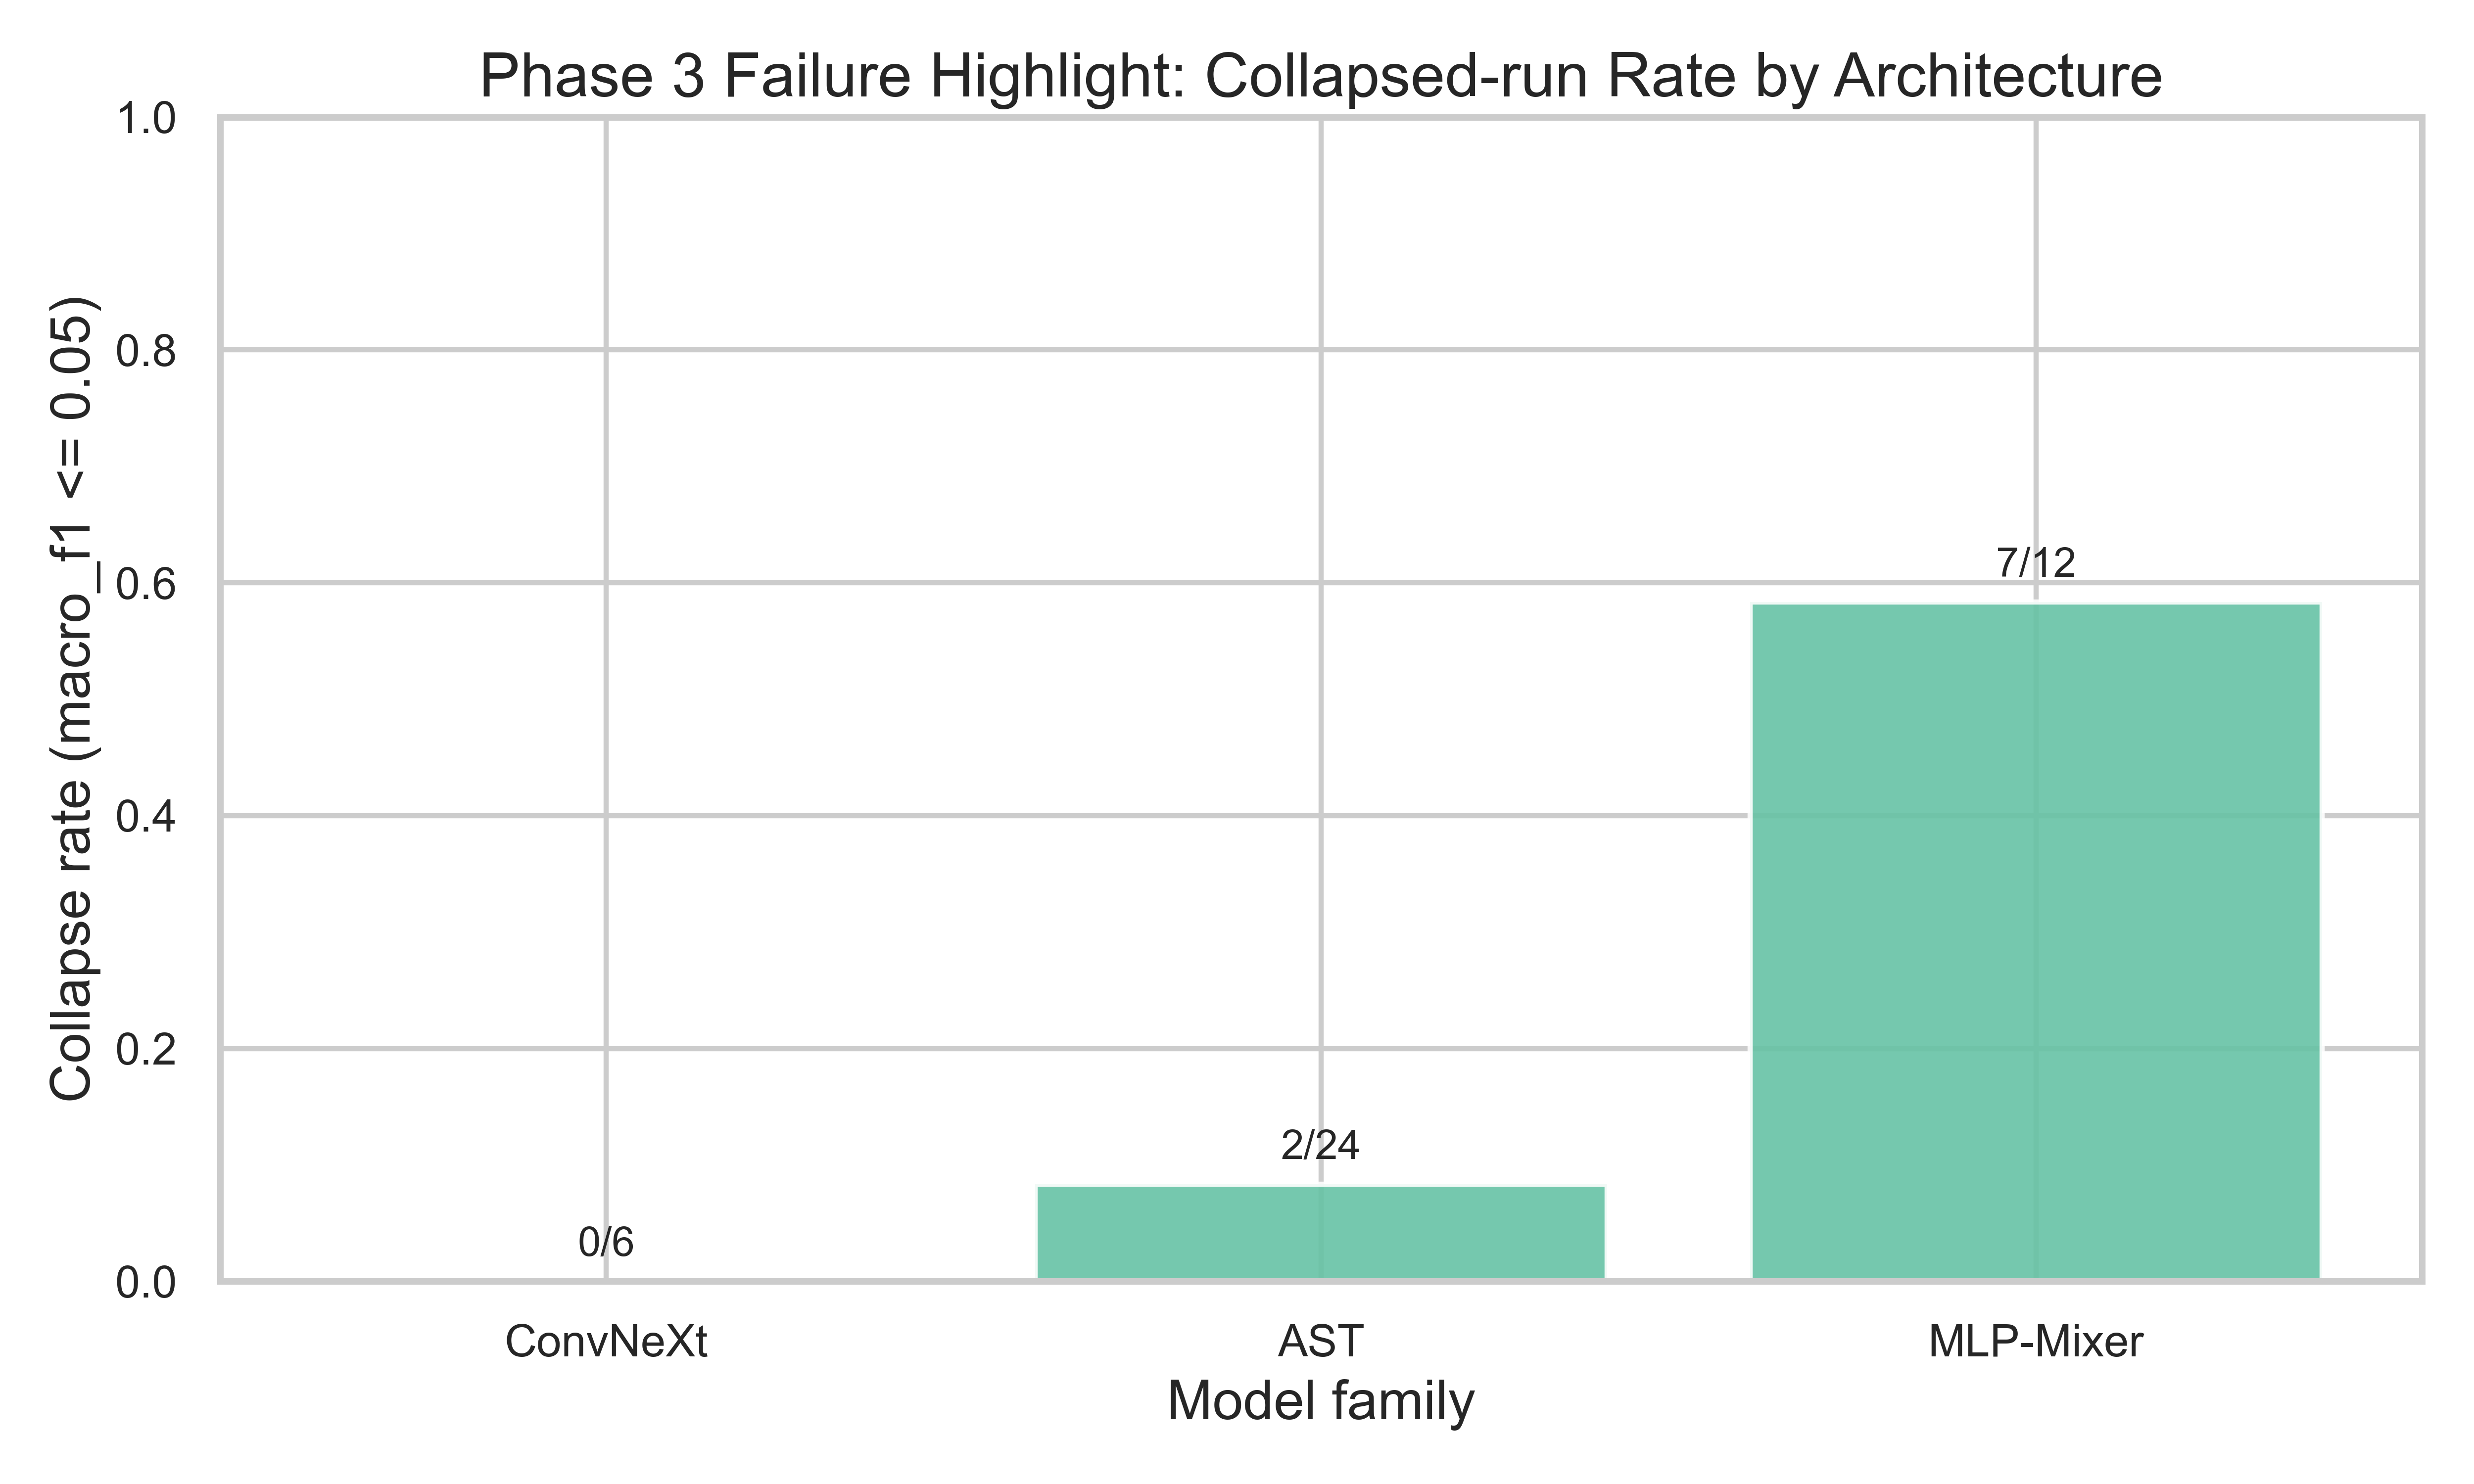
\includegraphics[height=0.68\textheight,keepaspectratio]{phase_3_failure_highlight.png}
    \slidecomment{Collapse-rate analysis confirms reliability differences: ConvNeXt has the fewest severe failures, MLP-Mixer the most.}
\end{frame}

\begin{frame}{Training Efficiency (ConvNeXt vs AST)}
    \centering
    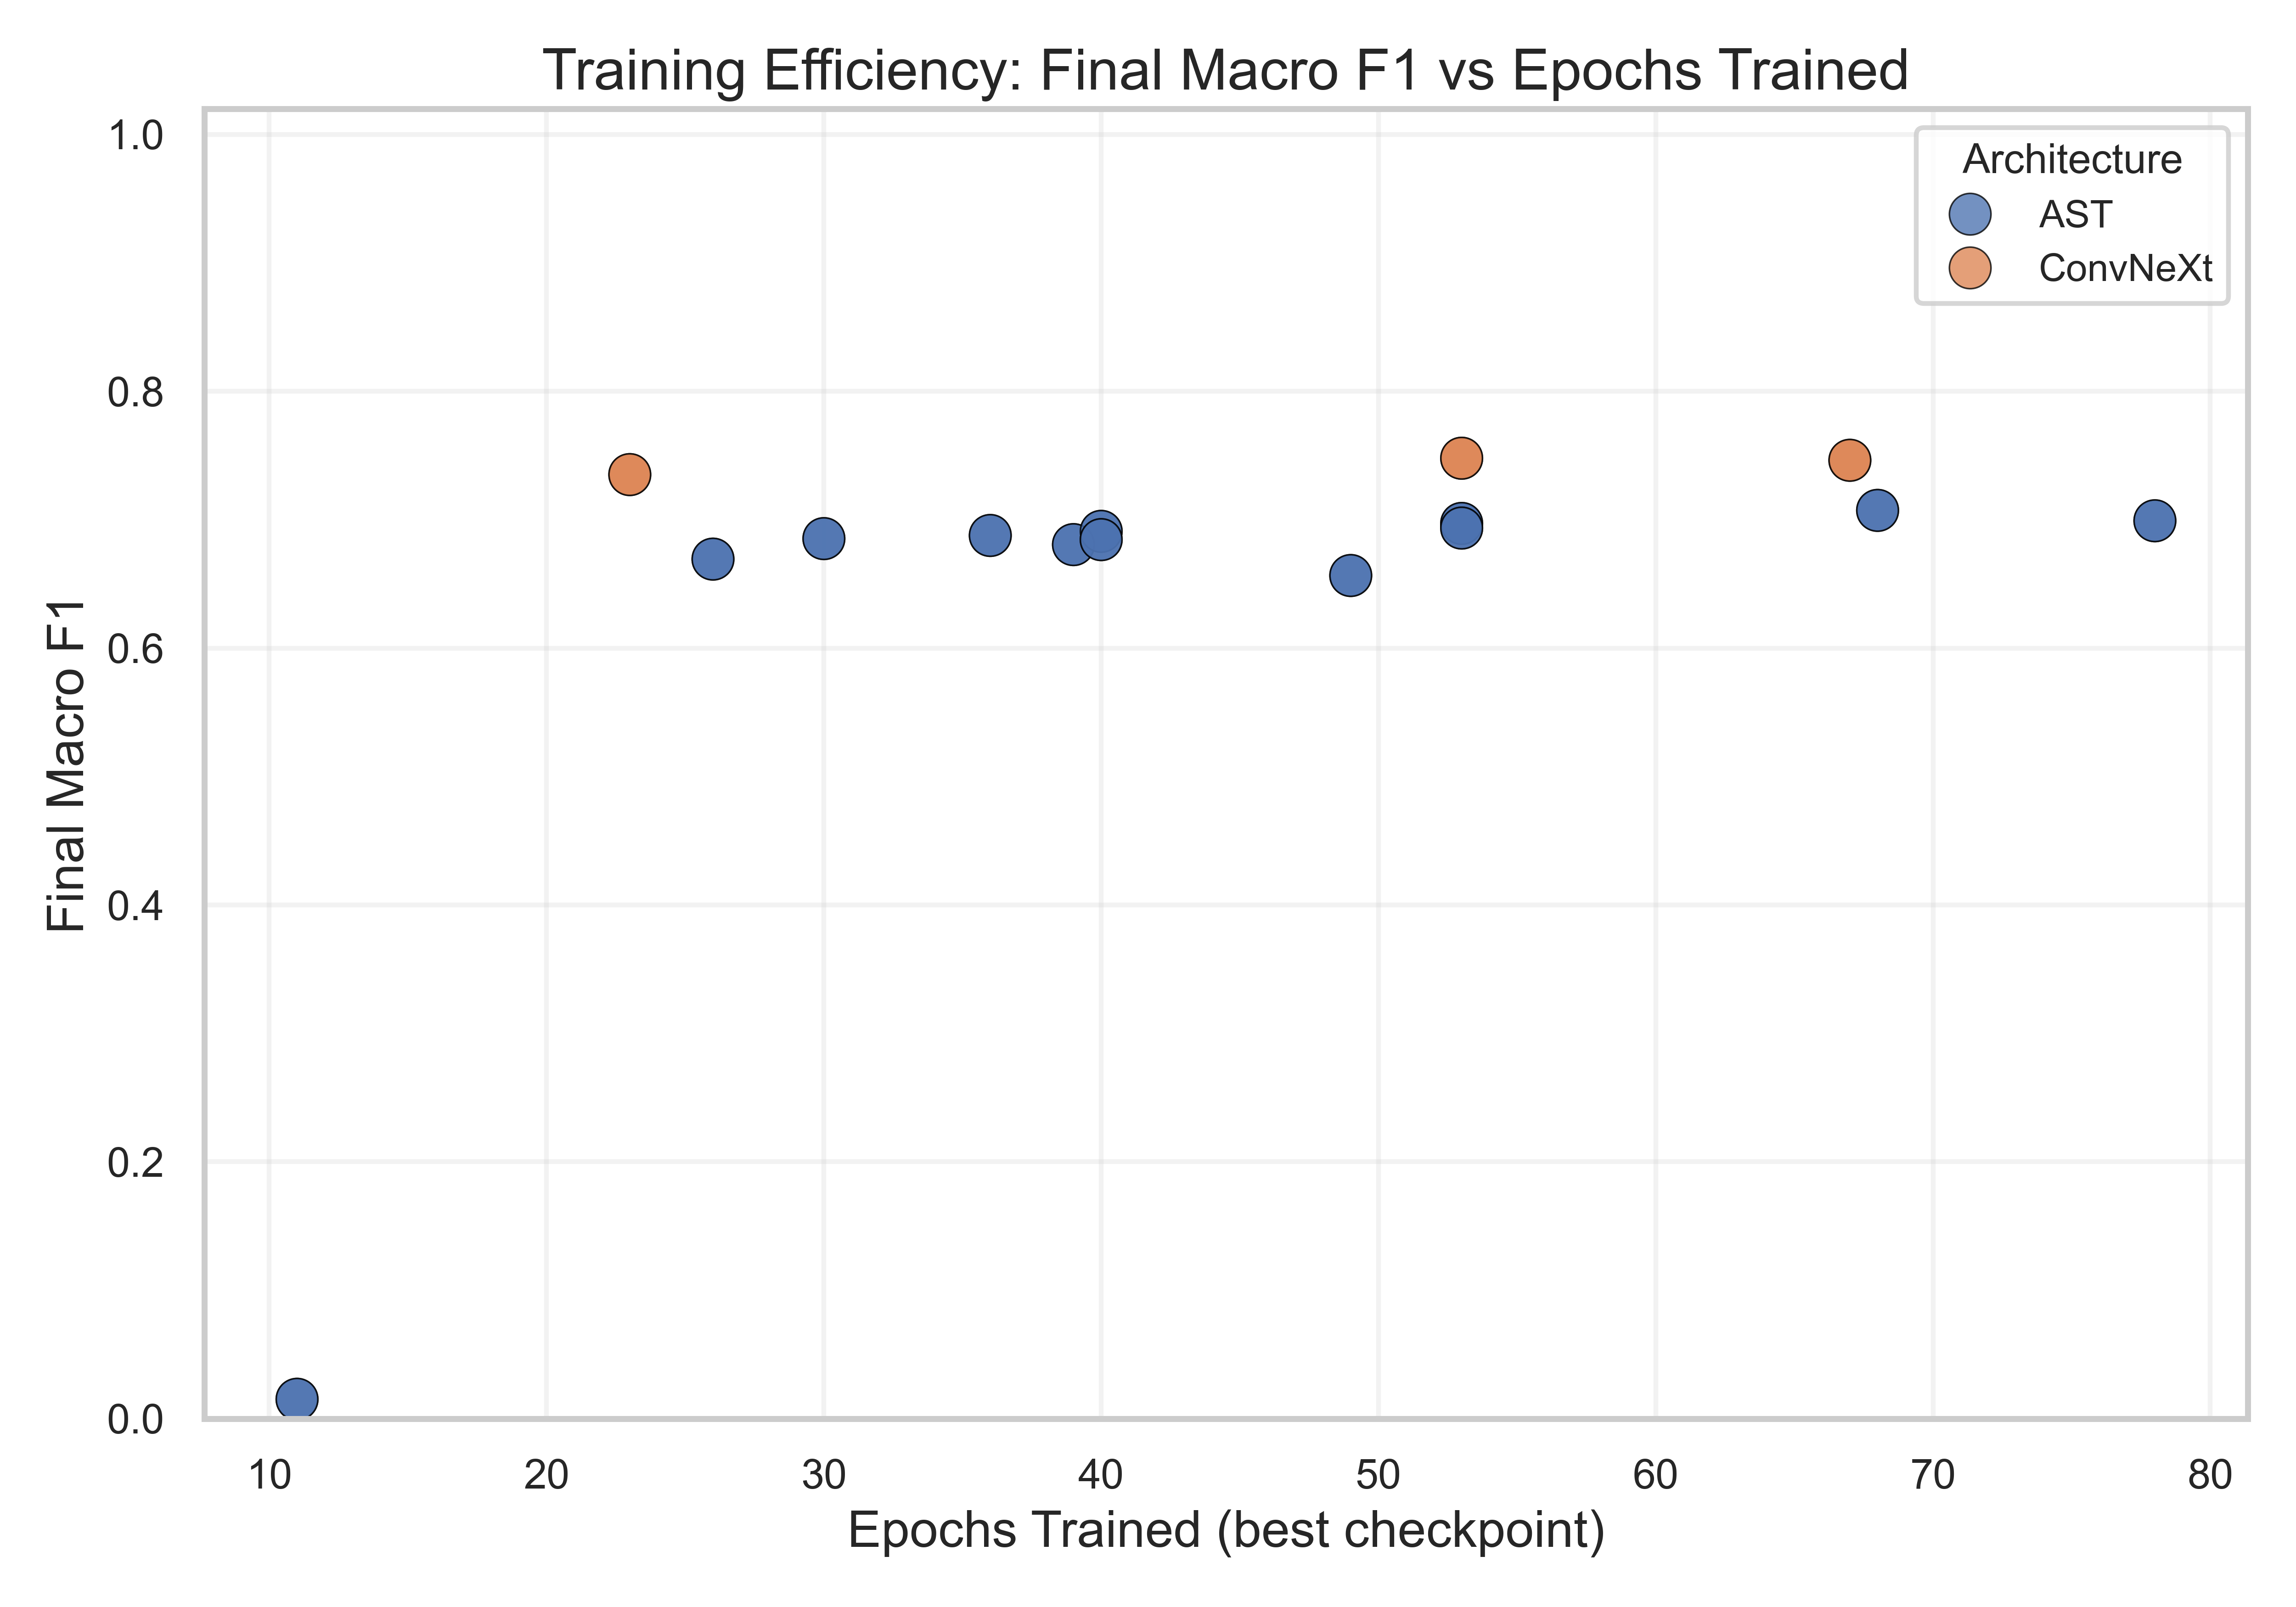
\includegraphics[height=0.68\textheight,keepaspectratio]{training_efficiency_scatter.png}
    \slidecomment{AST often converges in fewer epochs, but ConvNeXt achieves better mean and best-case final F1.}
\end{frame}

\begin{frame}{Phase 4: Open-Set Trade-off}
    \centering
    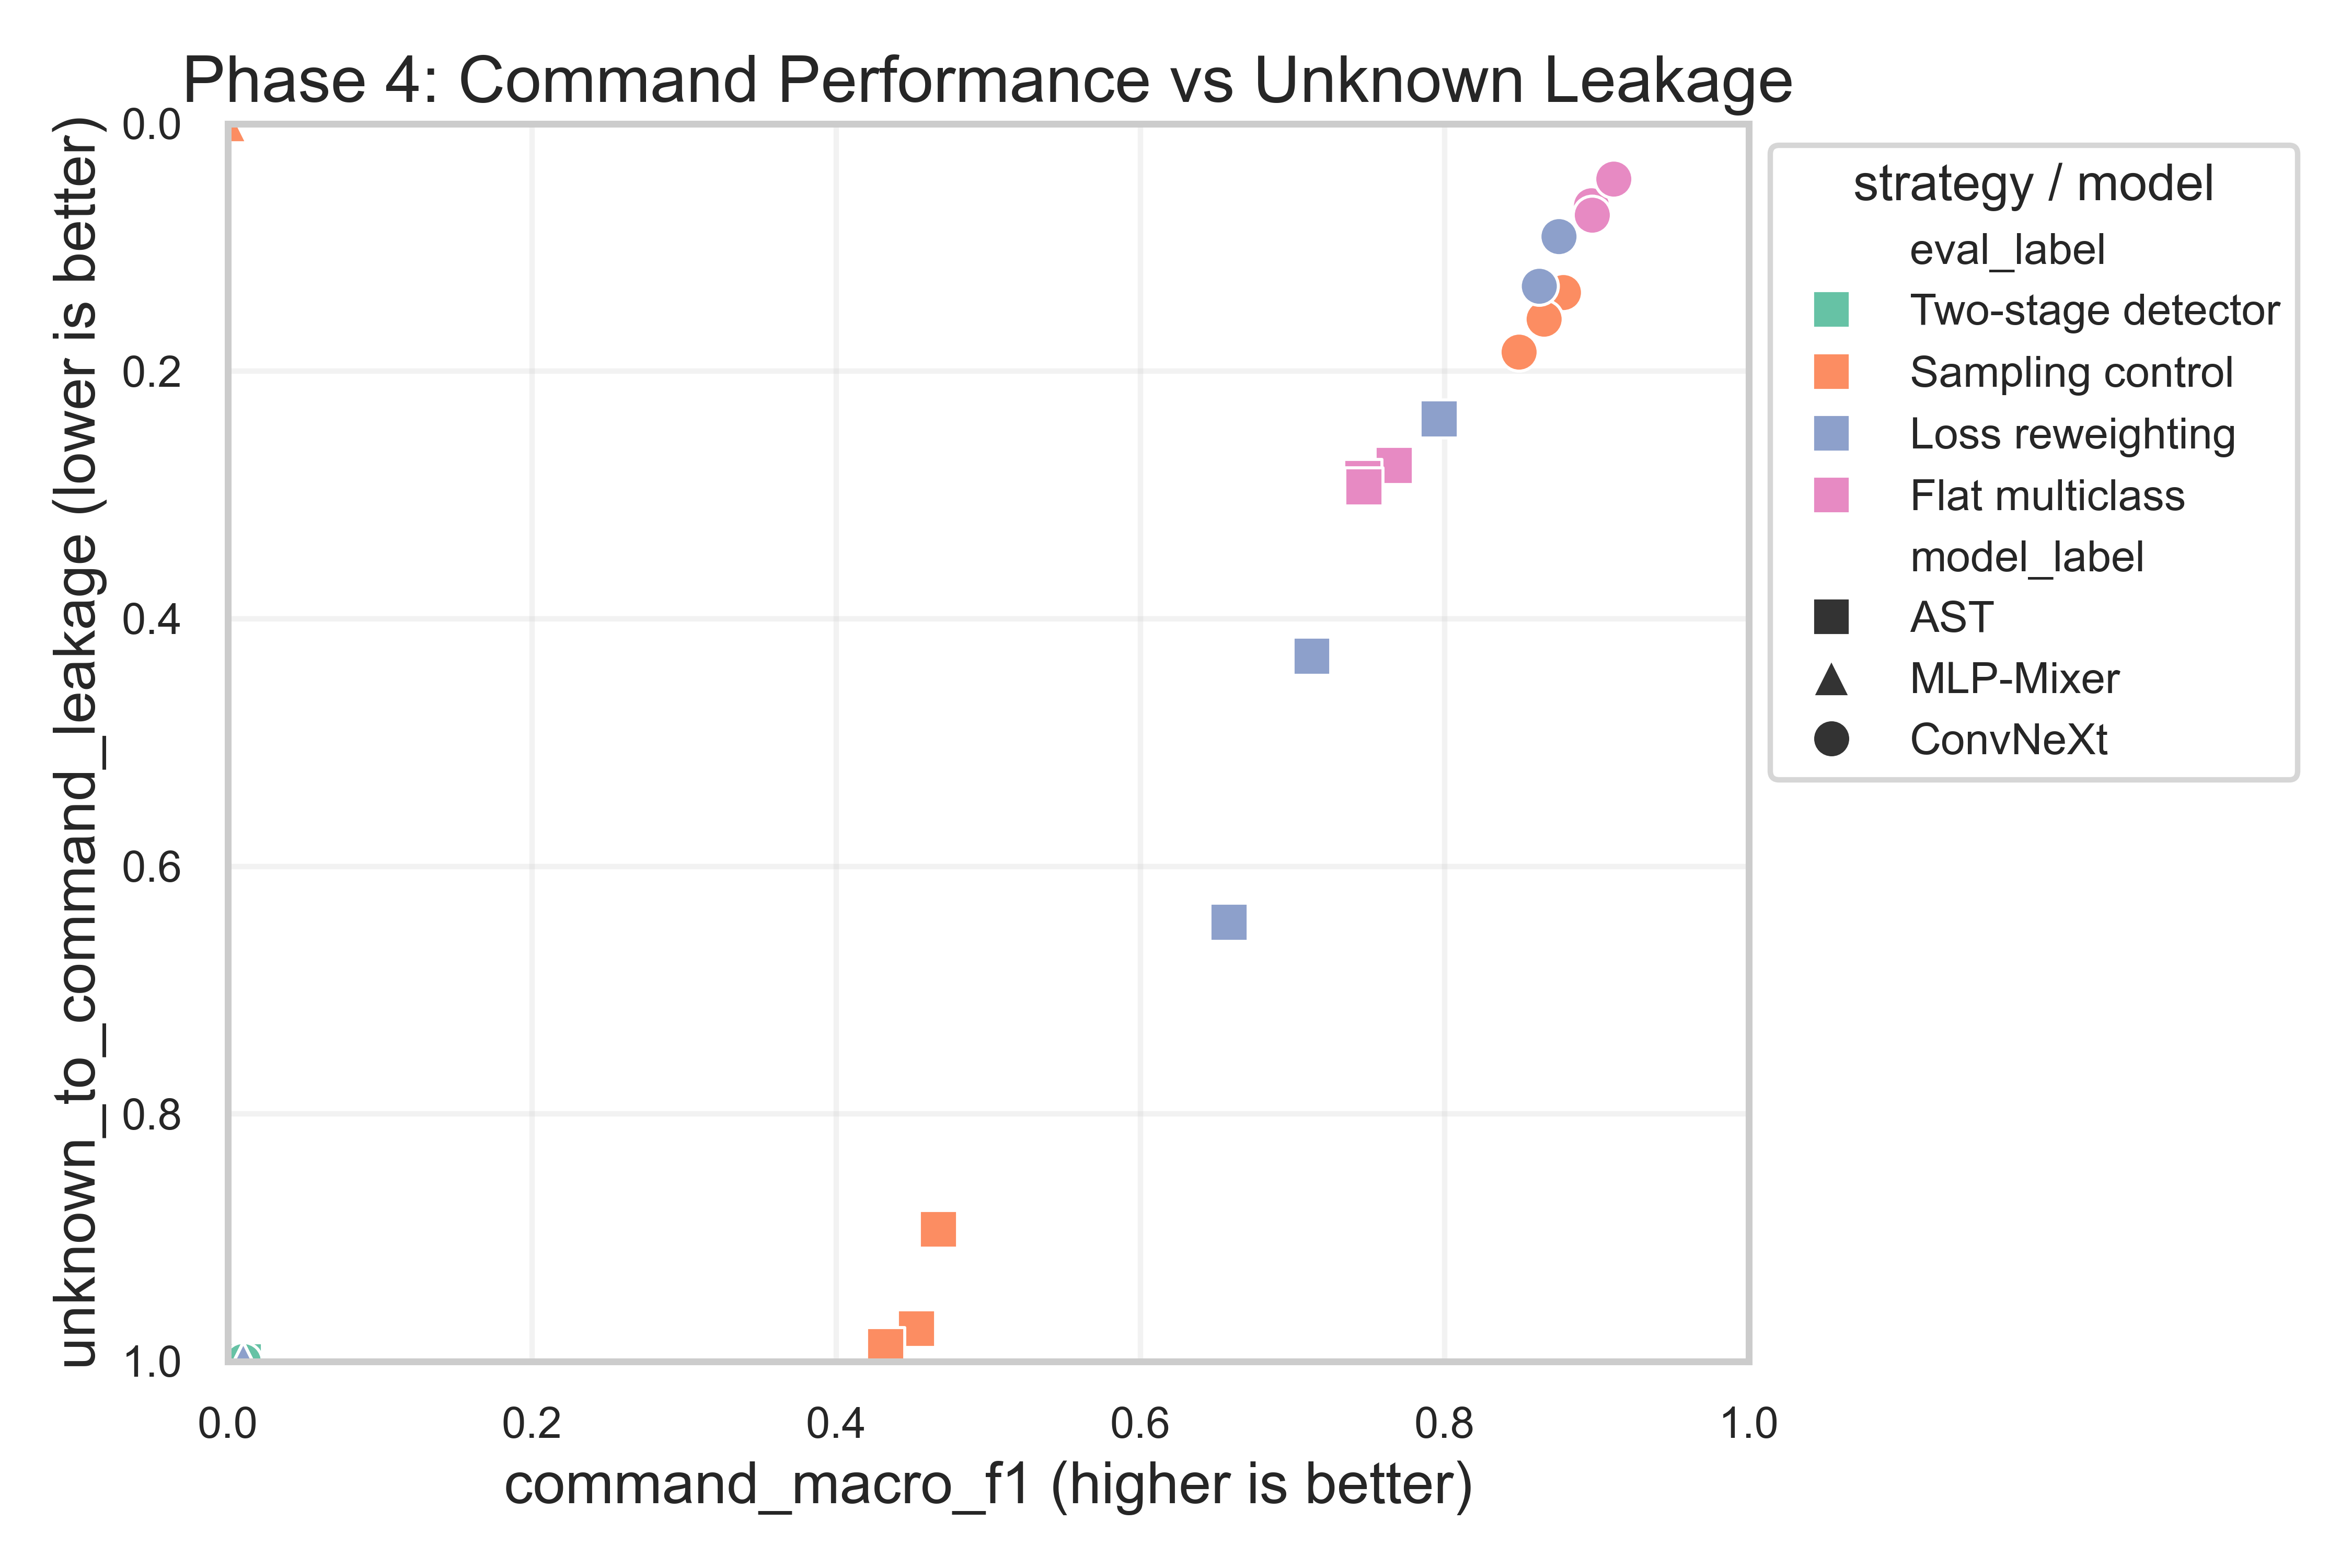
\includegraphics[height=0.68\textheight,keepaspectratio]{phase_4_pareto_scatter.png}
    \slidecomment{Flat multiclass and loss reweighting dominate the command-vs-leakage frontier; two-stage detector is not competitive.}
\end{frame}

\begin{frame}{Phase 4: Silence False Trigger Rate}
    \centering
    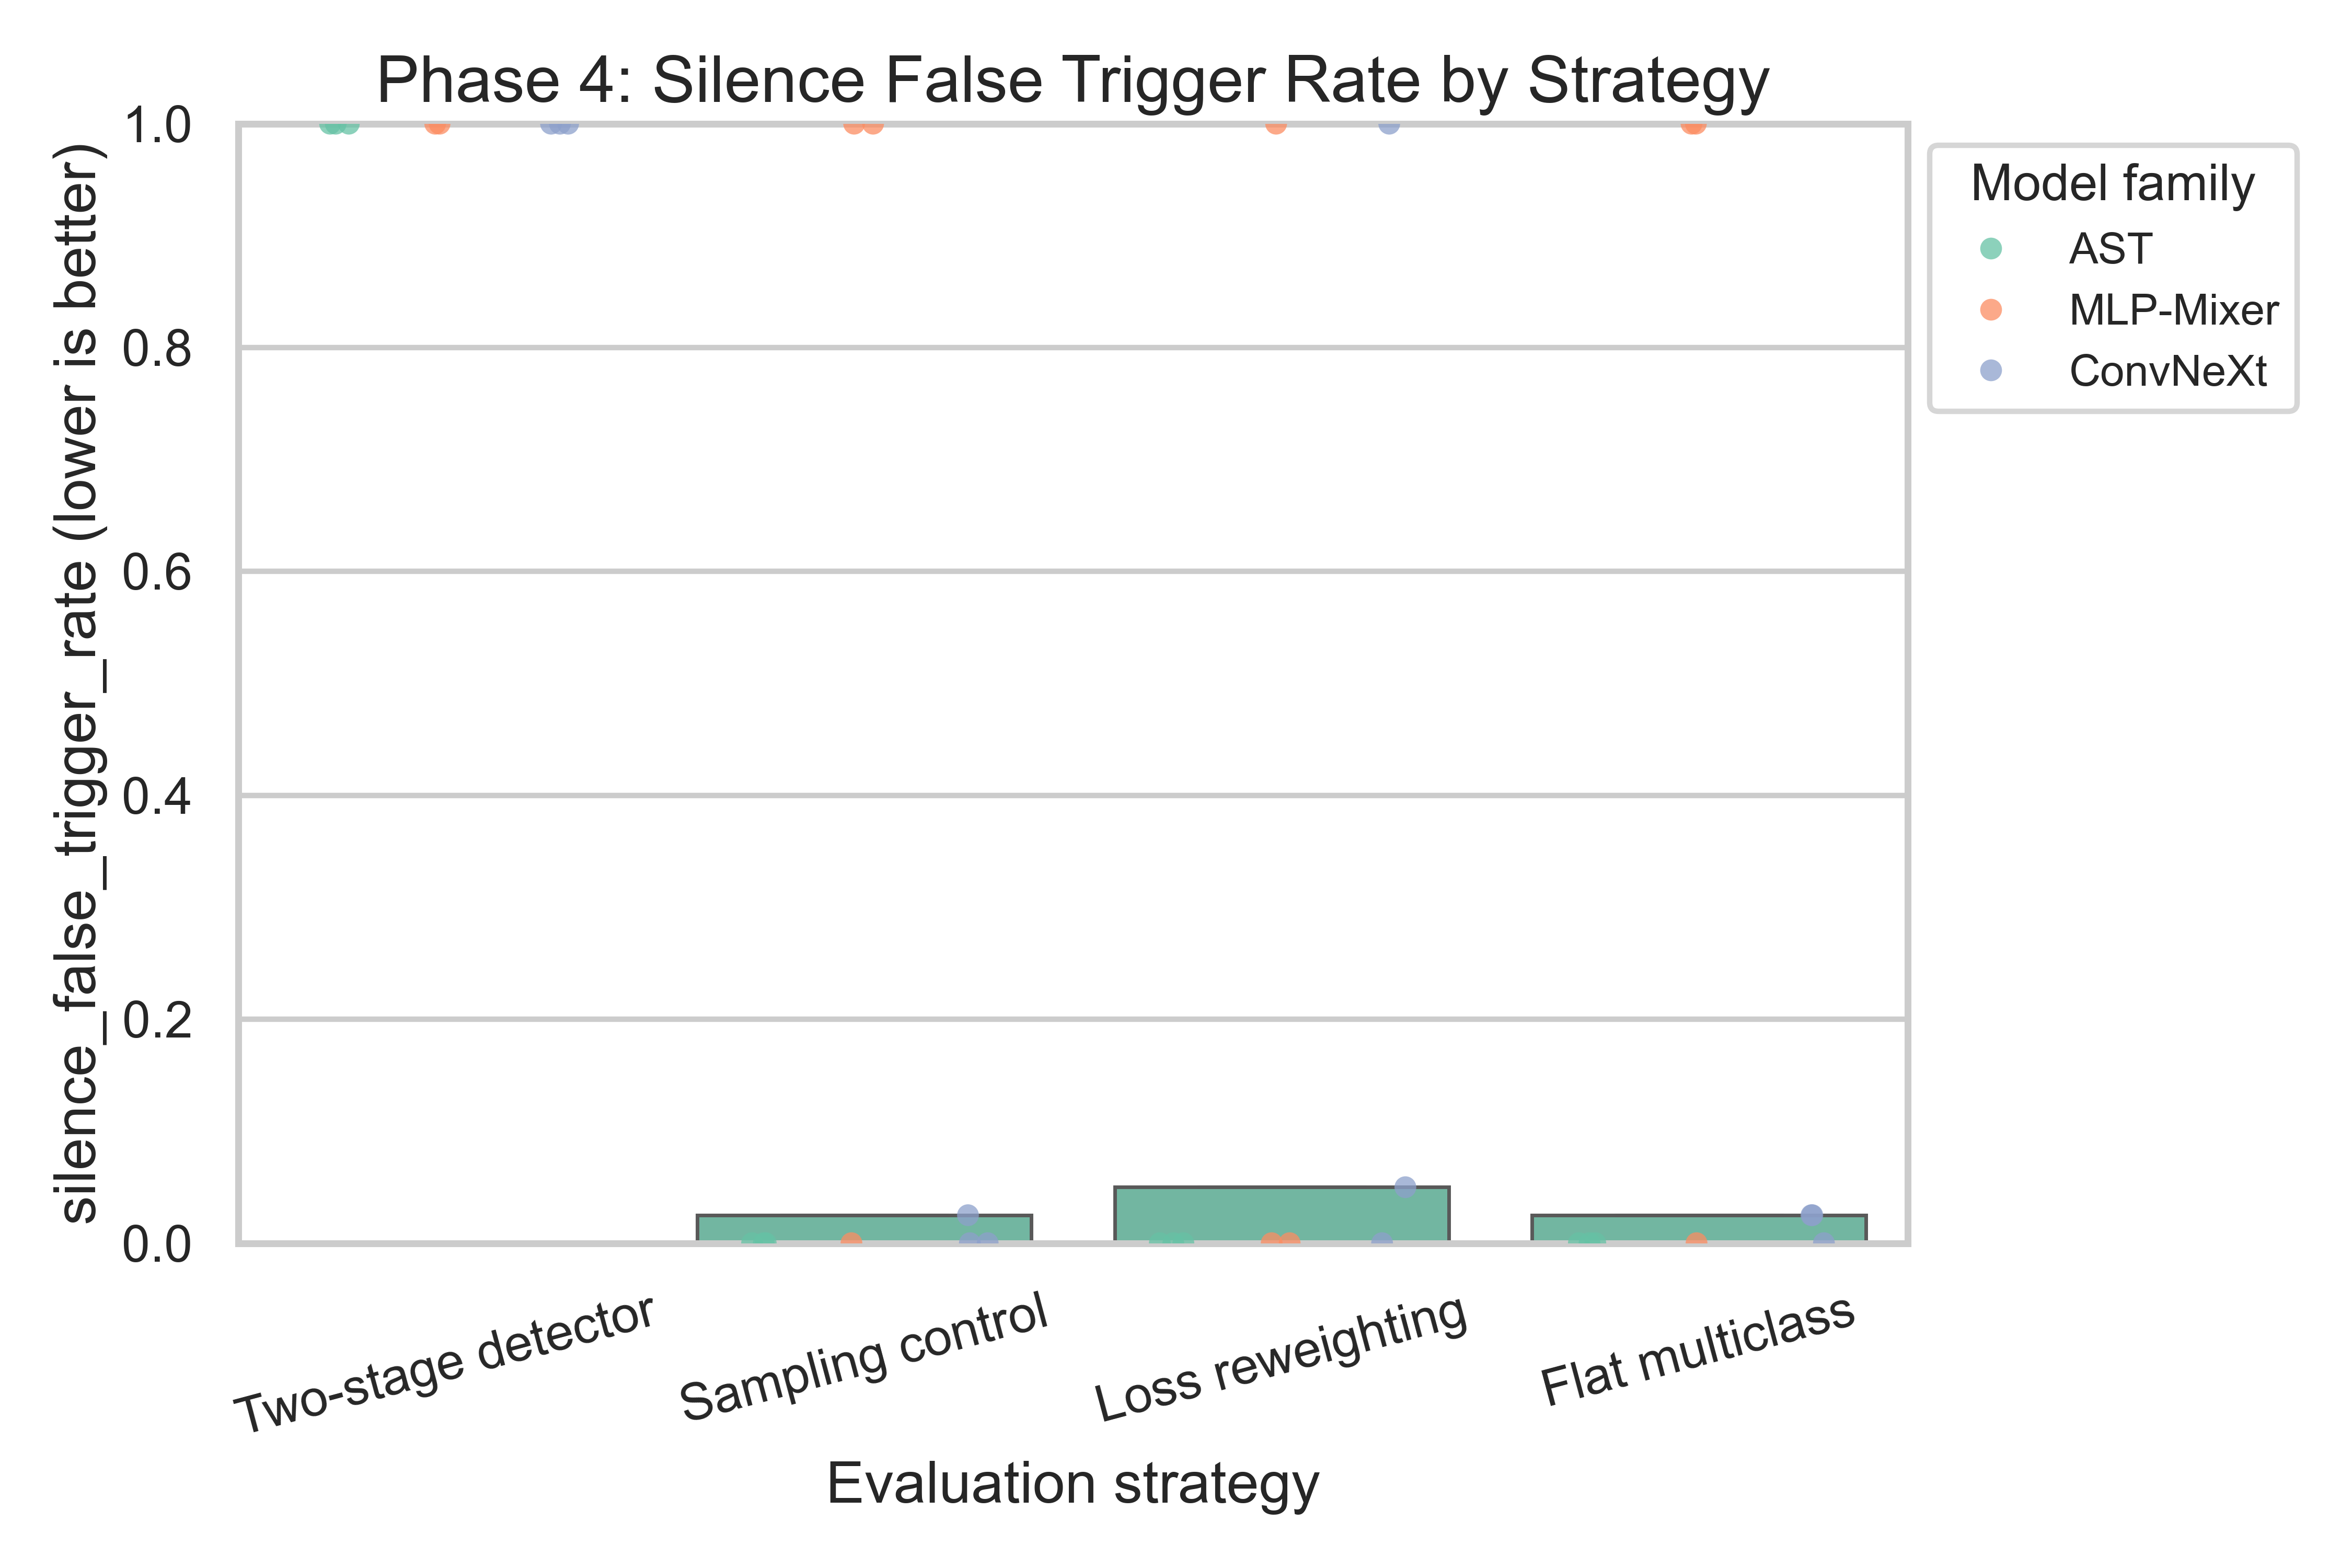
\includegraphics[height=0.68\textheight,keepaspectratio]{phase_4_silence_false_trigger_rate.png}
    \slidecomment{Two-stage detector shows a critical failure mode with elevated silence false triggers, which is unacceptable for always-on KWS.}
\end{frame}

\begin{frame}{Phase 4: Strategy Radar}
    \centering
    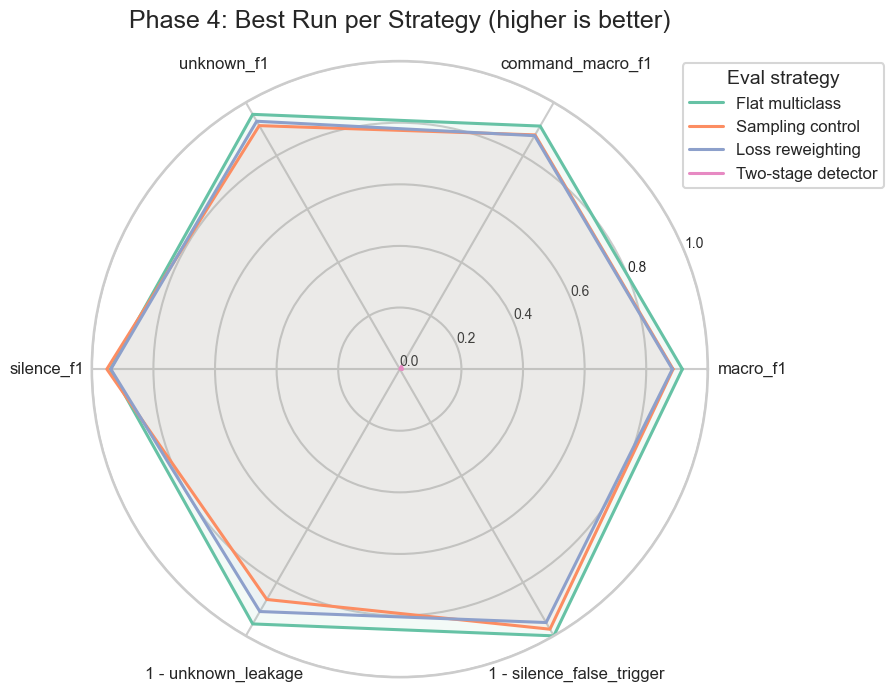
\includegraphics[height=0.68\textheight,keepaspectratio]{phase_4_strategy_radar.png}
    \slidecomment{Flat multiclass delivers the strongest overall deployment profile; sampling control can help but is less consistent across models.}
\end{frame}

\begin{frame}{Per-Class Best Model Diagnostics}
    \centering
    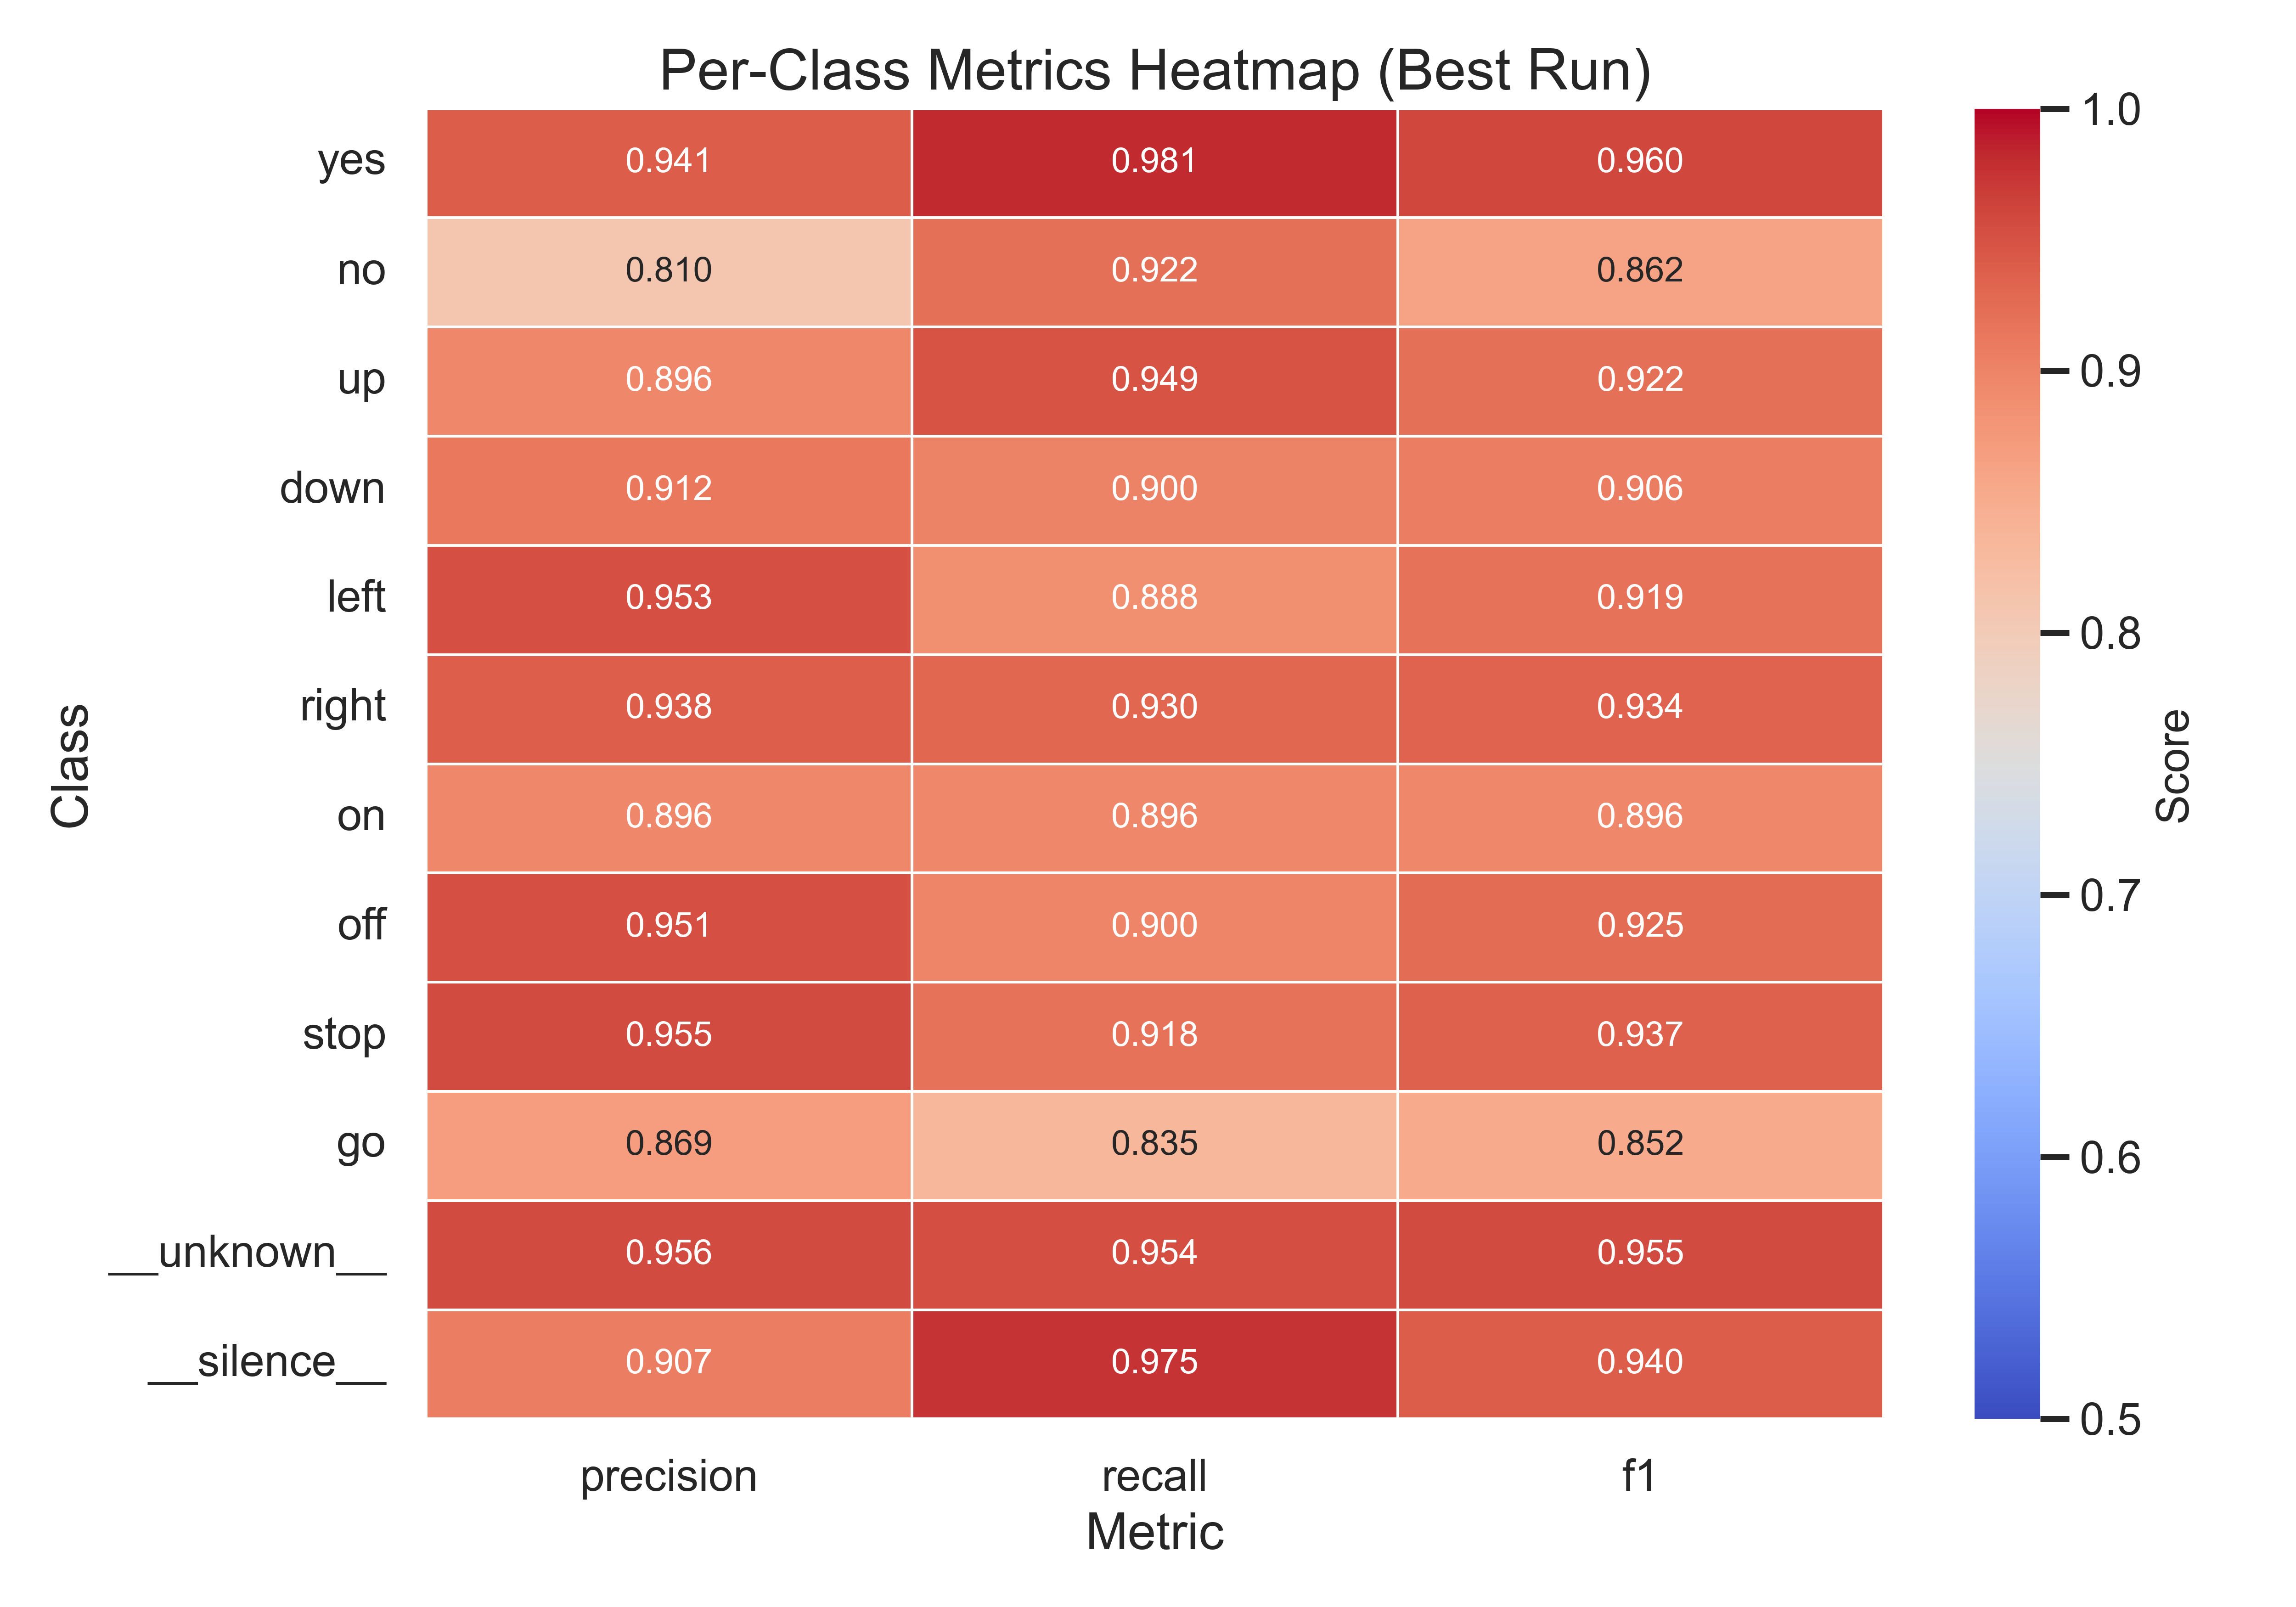
\includegraphics[height=0.68\textheight,keepaspectratio]{per_class_heatmap.png}
    \slidecomment{Residual errors concentrate on phonetically similar pairs (notably go and no), while unknown handling remains strong.}
\end{frame}

\section{Takeaways}

\begin{frame}{Final Conclusions}
    \begin{itemize}
        \item The 4-phase funnel provides a reproducible and practical KWS evaluation protocol.
        \item ConvNeXt is the best overall architecture under the shared from-scratch setup.
        \item Flat multiclass is the safest and strongest non-command handling strategy in this benchmark.
        \item Unknown leakage and silence false-trigger metrics are essential for deployment decisions, however performance is good.
        \item Future work: explore more architectures, larger datasets, and real-world robustness tests.
    \end{itemize}
\end{frame}

\begin{frame}[plain]
    \centering
    \Huge \textbf{Thank You}
    \vspace{1.2em}

    \large Questions?
    \vspace{1.2em}

    \normalsize
    Paweł Pozorski, Paweł Florek \\
    Warsaw University of Technology \\
    {\small \{pawel.pozorski, pawel.florek\}.stud@pw.edu.pl}
\end{frame}

\end{document}
